\documentclass[tikz,border=12pt]{standalone}
\usepackage[T1]{fontenc}
\usepackage{mathpazo}
\usepackage{amsmath,amssymb}
\usetikzlibrary{arrows.meta, positioning, calc, fit, decorations.pathreplacing}

\definecolor{stblue}{HTML}{7B97AD}
\definecolor{rwgold}{HTML}{B8995E}
\definecolor{sage}{HTML}{7A9A7E}
\definecolor{dkbrown}{HTML}{3D3530}
\definecolor{wmgray}{HTML}{7B7067}
\definecolor{cream}{HTML}{F9F6F0}
\definecolor{border}{HTML}{D4C9B8}
\definecolor{terracotta}{HTML}{C47A6A}
\definecolor{lavender}{HTML}{907EA0}

\begin{document}
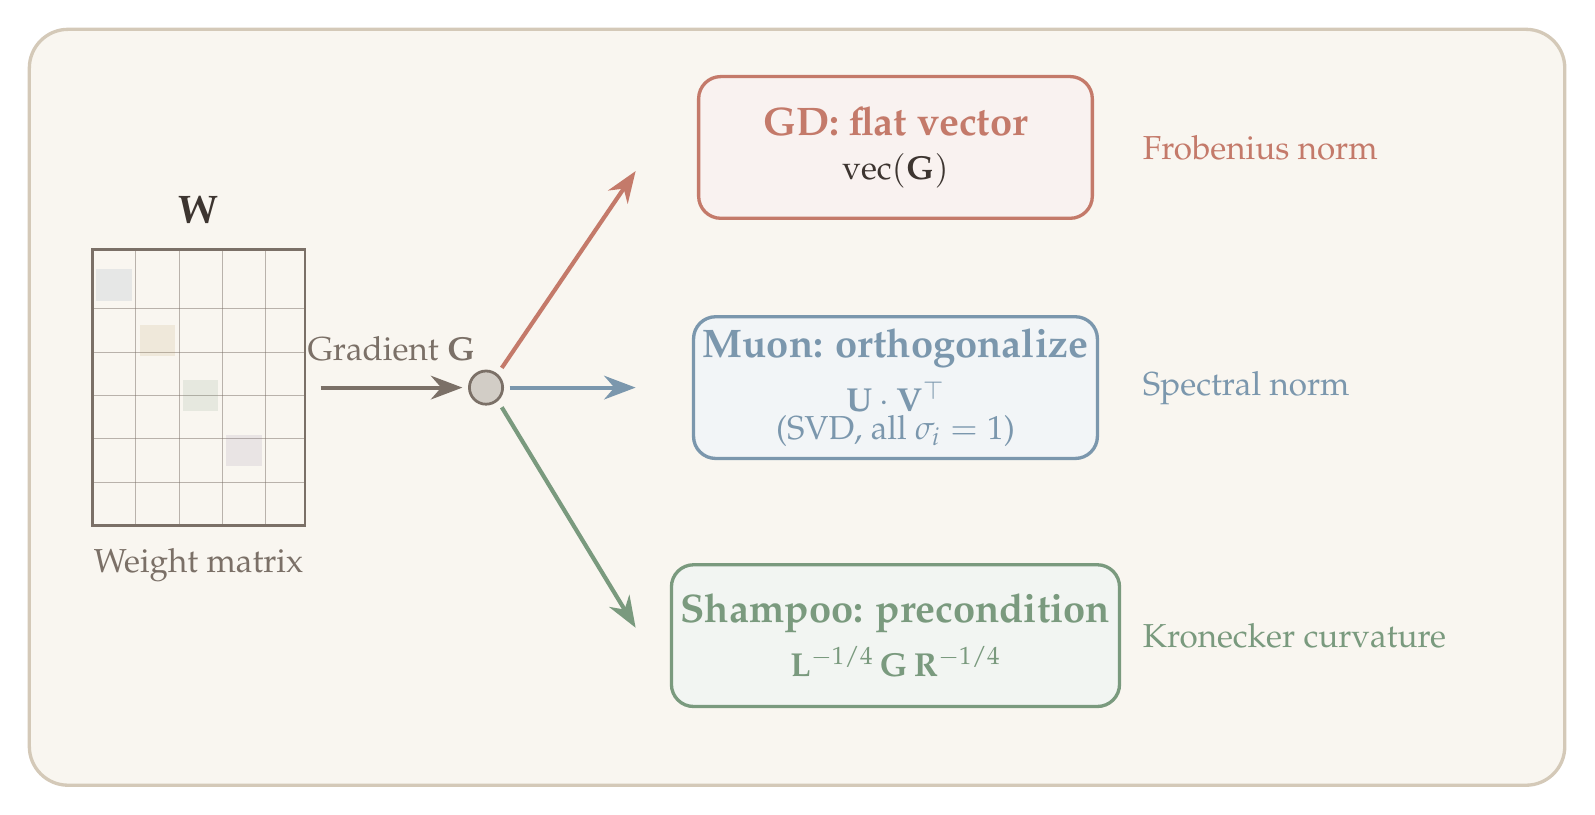
\begin{tikzpicture}[>={Stealth[length=4mm, width=3mm]}, line width=1.5pt]

% Background
\fill[cream, rounded corners=14pt] (-0.5,-0.8) rectangle (19.0,8.8);
\draw[border, line width=1.2pt, rounded corners=14pt] (-0.5,-0.8) rectangle (19.0,8.8);

% Weight matrix W grid
\draw[wmgray, line width=1pt] (0.3,2.5) rectangle (3.0,6.0);
\foreach \x in {0.85,1.4,1.95,2.5} {
  \draw[wmgray, line width=0.3pt, opacity=0.5] (\x,2.5) -- (\x,6.0);
}
\foreach \y in {3.05,3.6,4.15,4.7,5.25} {
  \draw[wmgray, line width=0.3pt, opacity=0.5] (0.3,\y) -- (3.0,\y);
}
% Cell fills
\fill[stblue, opacity=0.15] (0.35,5.35) rectangle (0.8,5.75);
\fill[rwgold, opacity=0.15] (0.9,4.65) rectangle (1.35,5.05);
\fill[sage, opacity=0.15] (1.45,3.95) rectangle (1.9,4.35);
\fill[lavender, opacity=0.15] (2.0,3.25) rectangle (2.45,3.65);

\node[text=dkbrown, font=\Large\bfseries] at (1.65,6.5) {$\mathbf{W}$};
\node[text=wmgray, font=\large] at (1.65,2.0) {Weight matrix};

% Arrow: Gradient G
\draw[wmgray, ->, line width=1.5pt] (3.2,4.25) -- (5.0,4.25);
\node[text=wmgray, font=\large] at (4.1,4.75) {Gradient $\mathbf{G}$};

% Branching node
\fill[wmgray, opacity=0.3] (5.3,4.25) circle (6pt);
\draw[wmgray, line width=1pt] (5.3,4.25) circle (6pt);

% Branch 1: GD (top)
\draw[terracotta, ->, line width=1.5pt] (5.5,4.5) -- (7.2,7.0);

\node[draw=terracotta, line width=1.2pt, fill=terracotta!10, rounded corners=8pt,
      minimum width=5.0cm, minimum height=1.8cm, align=center] (gd) at (10.5,7.3)
      {{\color{terracotta}\textbf{\Large GD: flat vector}}\\[4pt]
       {\large\color{dkbrown} $\mathrm{vec}(\mathbf{G})$}};

% Branch 2: Muon (middle)
\draw[stblue, ->, line width=1.5pt] (5.6,4.25) -- (7.2,4.25);

\node[draw=stblue, line width=1.2pt, fill=stblue!10, rounded corners=8pt,
      minimum width=5.0cm, minimum height=1.8cm, align=center] (muon) at (10.5,4.25)
      {{\color{stblue}\textbf{\Large Muon: orthogonalize}}\\[4pt]
       {\large\color{stblue} $\mathbf{U} \cdot \mathbf{V}^\top$}\\[-2pt]
       {\large\color{stblue} (SVD, all $\sigma_i = 1$)}};

% Branch 3: Shampoo (bottom)
\draw[sage, ->, line width=1.5pt] (5.5,4.0) -- (7.2,1.2);

\node[draw=sage, line width=1.2pt, fill=sage!10, rounded corners=8pt,
      minimum width=5.0cm, minimum height=1.8cm, align=center] (shampoo) at (10.5,1.1)
      {{\color{sage}\textbf{\Large Shampoo: precondition}}\\[4pt]
       {\large\color{sage} $\mathbf{L}^{-1/4}\,\mathbf{G}\,\mathbf{R}^{-1/4}$}};

% Right-side summary labels
\node[text=terracotta, font=\large, anchor=west] at (13.5,7.3) {Frobenius norm};
\node[text=stblue, font=\large, anchor=west] at (13.5,4.25) {Spectral norm};
\node[text=sage, font=\large, anchor=west] at (13.5,1.1) {Kronecker curvature};

\end{tikzpicture}
\end{document}
